\documentclass{article}
\setlength{\headheight}{33pt}

\usepackage[
  top=1.8cm,
  bottom=1.5cm,
  left=1.8cm,
  right=1.8cm,
  includefoot,
  includehead]{geometry}

\usepackage[utf8]{inputenc}
\usepackage{changepage}
\usepackage{multicol}
\usepackage{nccmath}
\usepackage{amsmath}
\usepackage{graphicx}
\usepackage{calc}
\usepackage{enumitem}

% For fancy math
\RequirePackage{amsmath,amsthm,amssymb}
\newtheorem{theorem}{Theorem}
\newtheorem{fact}[theorem]{Fact}
\newtheorem{lemma}[theorem]{Lemma}
\newtheorem{claim}[theorem]{Claim}

\newcommand{\ord}[2][th]{\ensuremath{{#2}^{\mathrm{#1}}}}
% shorthand for \mathcal{O}
\newcommand{\Ocal}{\ensuremath{\mathcal{O}}}
\newcommand{\aug}{\fboxsep=-\fboxrule\!\!\!\fbox{\strut}\!\!\!}
\newcommand{\contradiction}{%
  \ensuremath{{\Rightarrow\mspace{-2mu}\Leftarrow}}%
}

\graphicspath{{./images}}

% Counters for HW number, author, and collaborators
\newcommand{\hwnumber}[1]{\def\hwnumberdata{#1}}
\def\hwnumberdata{\relax}
\renewcommand{\author}[1]{\def\authordata{#1}}
\def\authordata{\relax}
\newcommand{\collaborators}[1]{\def\collaboratorsdata{#1}}
\def\collaboratorsdata{\relax}

% Fancy headings
\RequirePackage{fancyhdr}
\pagestyle{fancyplain}

\fancyhead[L]{\small \authordata \\
\small CS 630 Homework \#\hwnumberdata \\
  \textsl{Collaborators}: \collaboratorsdata}

\RequirePackage{titlesec}
\titleformat{\subsection}{\normalsize\bfseries}{\thesubsection}{.5em}{}
\renewcommand{\thesubsection}{\alph{subsection})}

% Making the problem and ppart environments
\newcommand{\addmedskip}{\addvspace{2\medskipamount}}
\newcommand{\addbigskip}{\addvspace{2\bigskipamount}}
\newcommand{\nline}{\bigskip}

\newcounter{problemnum}
\setcounter{problemnum}{0}
\newenvironment{problem}
  {\addbigskip \setcounter{partnum}{0}
   \noindent\stepcounter{problemnum}\textbf{Problem \arabic{problemnum}.\ }}
  {\par\addbigskip}

\newcounter{partnum}
\setcounter{partnum}{0}

\newenvironment{ppart}[1][]{%
  \addmedskip
  \refstepcounter{partnum}%\par\medskip%
  \enumerate[labelsep=*]\item[\textbf{\roman{partnum})}]}
  {\endenumerate}

\newsavebox{\mybox}
\newenvironment{answer}
{\begin{lrbox}{\mybox}\begin{minipage}{0.95\textwidth}\vspace{0.2cm}}
  {\vspace{0.1cm}\end{minipage}\end{lrbox}\fbox{\usebox{\mybox}}}

\newenvironment{customProof}{\begin{proof}\noindent}{\end{proof}}

% Put your name and the homework number here.
\author{Jiun-Yan (Eric) Chen}
\hwnumber{4}


\begin{document}
\vspace*{0.5\baselineskip}
\textbf{Please limit your answer to the following problems to at most 1/2 a page each.}

\collaborators{None} % Put your collaborators for the problem here
\begin{problem}
    Consider the graphs G given.

    \begin{ppart}
        State the size of the min-cut G, state how many min cuts G has and list them. What is the size of thet max cut of G. List all of G's max-cuts.
    \end{ppart}

    \begin{answer}
        Min-Cuts:
        
        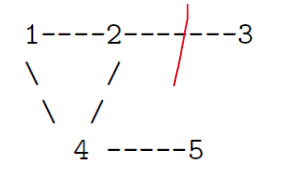
\includegraphics[scale=0.5]{1-1.png}

        Max-Cuts:

        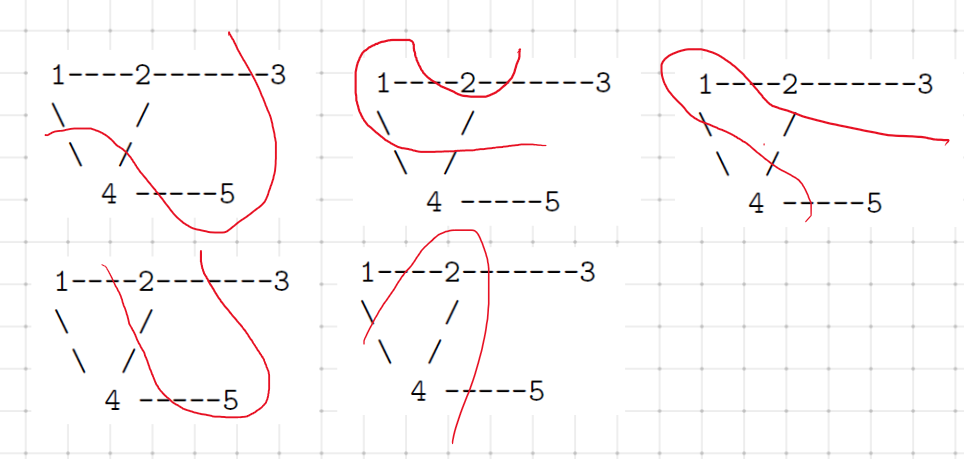
\includegraphics[scale=0.5]{1-2.png}

        The min-cut size is 1, and there are 2 min-cuts, the max-cut size is 4.
    \end{answer}

    \begin{ppart}
        Compute the exact probability that the algorithm will find a min cut of graph G after running the contraction algorithm once. Show your work in doing this computation.
    \end{ppart}

    \begin{answer}
         Probability of last contraction being 2-3 or 4-5 is $4! \times 2 / 5! = \frac{2}{5}$
    \end{answer}
\end{problem}

\newpage

\collaborators{None} % Put your collaborators the problem here
\begin{problem}

    \begin{ppart}
        Prove that the maximum number of min-cuts that a graph of n vertices can have is $\Ocal(n(n-1)/2)$.
    \end{ppart}

    \begin{answer}
       The probability of the Randomize Min-Cut algorithm of finding a min-cut is $2/(n(n-1))$.

       \hrulefill
       
        Proof:
    
        If a graph has a min-cut of size k, than each vertex must have a minimum degree of k. Therefore the amount of edges that the graph can have is $|E| >= \frac{kn}{2}$.

        For a min-cut, the probability of a contraction not being an edge in the min-cut is 
        
        $1 - \frac{k}{|E|} >= 1 - \frac{2}{n}$. For each additional step i, the conditional probability of the new edge not being a min-cut $Pr >= 1 - \frac{2}{n-i}$

        Therefore, the probability of success $Pr = (1 - \frac{2}{n})(1 - \frac{2}{n-1})(1 - \frac{2}{n-2})...(1 - \frac{2}{3}) >= \frac{2}{n(n-1)}$

        \hrulefill

        Since for each min-cut, there is a $\frac{2}{n(n-1)}$ probabilty of the algorithm succeeding, there must be at most $1 / \frac{2}{n(n-1)} = \frac{n(n-1)}{2}$ min-cuts, as the sum of the probability is bound to 1. 
        
        (Can be summed because each min-cut's probability is independent of one another)
    \end{answer}

    \begin{ppart}
        Give an example of a graph of at least $k > 5$ vertices which has at least k(k-1)/2 min-cuts.
    \end{ppart}

    \begin{answer}
        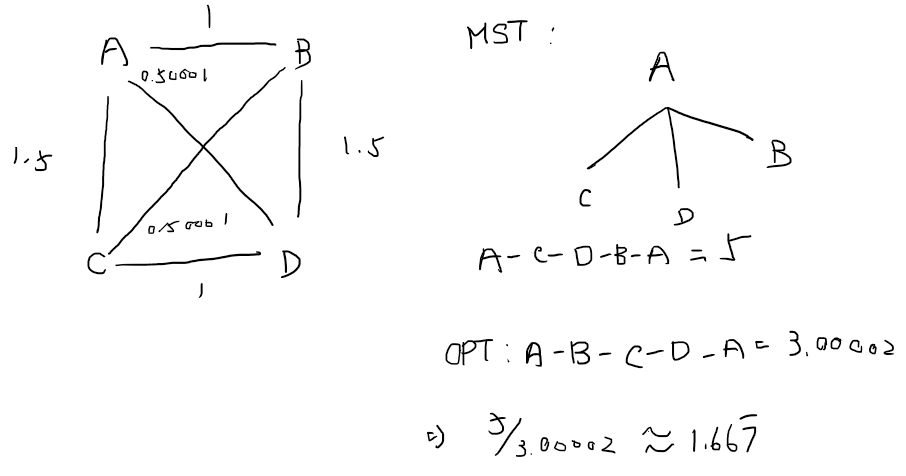
\includegraphics[scale=0.5]{2-2.png}
    \end{answer}
\end{problem}

\newpage

\begin{problem}
    Assume you have a list of N, $N > 10,000$, numbers from 1 to 100 and you know that more that .7 of the N numbers are the same (say T)

    \begin{ppart}
        Write a Monte Carlo algorithm which determines the number T with high probability

        Specifically your algorithm should,

        - run for some constant number of steps not depending on N, and

        - output the value T with probability at least .8

        You should state the time complexity and error bounds of your algorithm and explain why your algorithm achieves these times and error bounds.
    \end{ppart}
    \begin{answer}
        Pick k random number from the list. T is the number that appears the most often.

        The probability of this being wrong decreases with a higher k. 

        The worst case scenario is 0.7 of the list is T, and 0.3 is another number S.

        The probability of getting it wrong is the poisson distribution equation 
        
        $Pr = \sum^{k/2}_{i=0} \binom{k}{i} 0.7^i 0.3^{k-i}$

        Thus $Pr > 0.8$ when $k >= 8$. 
        
        Thus if k = 8, our algorithm will have a probability of being correct at least $80\% $ of the time


    \end{answer}

    \begin{ppart}
        Is it possible to find an efficient Las Vegas algorithm to solve this problem? That is, is there an algorithm which never makes an error and which finds the majority element in expected time $\Ocal(log N)$. Why or why not? Explain your reasoning.
    \end{ppart}

    \begin{answer}
        There is no Las Vegas algorithm capable that works in $\Ocal(logN)$ time.

        Any random sampling algorithm will always have a chance of picking numbers that are not the majority. This probability can be reduced by increasing the sampling amount, up to $0.3N + 1$ samplings with the lowest error rate (0\%). However, as the size of the list grows, the sampling requirements also increases to keep it at 0\% at $\Ocal(N)$ time. Thus, there is no algorithm that can never make an error and also complete in $\Ocal(logN)$ time.
    \end{answer}

\end{problem}

\newpage

\begin{problem}
    Let's slightly change the randomized min-cut algorithm discussed in class as follows: Instead of choosing an edge to contract, we randomly choose 2 vertices (which may or may not be connected by any edge) and contract them into 1 vertex by contracting them into a single vertex.

    Show that there are input graphs for which this new min-cut algorithm finds a min-cut with only exponentially small probability. That is, describe a specific graph with n vertices for which the contraction algorithm is likely to run for exponentially many iterations (in n) before it finds the min-cut in the graph. Explain your reasoning.
\end{problem}

\begin{answer}
    Take a graph G, where there are two n-complete graphs g1, g2, and a single edge between one vertex of g1 and g2 (lets call them i, j). The min-cut of this graph must be the cut on the edge between i and j

    \nline

    The algorithm will error out whenever it contracts vertices where one belongs in g1 and one belongs in g2.

    \nline

    As there are  a total of 2n vertices, there will need to be 2n-2 contractions. (n-1 for g1, g2 each.)

    \nline

    The chance of picking correct is therefore $Pr = \frac{(n-1)!(n-1)!}{2n!/2} = \frac{2 (n-1)(n-2)(n-3)...(n-n+1)}{(2n)(2n-1)(2n-2)...(2n-n+1)(2n-n)} \approx \frac{1}{n^2 \times 2^n}$, 

    \nline

    Thus, we have shown that there is at least one type of graph in which the algorithm has an exponentially small probability of getting the correct min-cut.

    \nline

    This is different to the original algorithm because there is only the single edge between i and j that will cause an error if contracted.
\end{answer}

\end{document}
